% Digest template for Intermag

\documentclass[journal,transmag]{IEEEtran}


\usepackage{cite}
\usepackage{graphicx}
\usepackage{amssymb,amsmath}

\usepackage{mathrsfs}
\usepackage{booktabs}

\usepackage{wasysym}


% correct bad hyphenation here
\hyphenation{mag-netic}


\begin{document}

% paper title
\title{Frequency-Domain Propagation in Multiconductor \\Submarine Power Cables}



% author names and affiliations
% transmag papers use the long conference author name format.


\author{
	\IEEEauthorblockN{Rooney R. A. Coelho\IEEEauthorrefmark{1}, Gabriel de Castro Biage\IEEEauthorrefmark{1}, Mario Leite P. Filho\IEEEauthorrefmark{2} and José Roberto Cardoso\IEEEauthorrefmark{1},~\IEEEmembership{Member,~IEEE}}
	\IEEEauthorblockA{\IEEEauthorrefmark{1}InnovaPower - RCGI, University of São Paulo, São Paulo, Brazil, \{rooneycoelho, gabriel.biage, jose.cardoso\}@usp.br}
	\IEEEauthorblockA{\IEEEauthorrefmark{2}Institute for Technological Research - IPT, São Paulo, Brazil, mleite@ipt.br}% <-this % stops an unwanted space
}



\IEEEtitleabstractindextext{%
\begin{abstract}
A comprehensive formulation for analyzing subsea cables in the frequency domain is introduced. This cable design encompasses multiple conductors, necessitating the resolution of a complex, coupled wave equation. To ensure accuracy and reliability, the derived results were rigorously validated against simulations conducted using PSCAD software.
\end{abstract}

\begin{IEEEkeywords}
Frequency Domain Analysis, Electromagnetic Wave Propagation, Subsea Cable Systems.
\end{IEEEkeywords}}


% make the title area
\maketitle

% no page numbering, or other headers / footers
\pagestyle{empty}
\thispagestyle{empty}

\IEEEpeerreviewmaketitle


\section{Introduction}
% The very first letter is a 2 line initial drop letter followed
% by the rest of the first word in caps.

\IEEEPARstart{S}{ubmarine cables} are crucial for transferring energy in marine environments, powering offshore renewable energy sources like wind, wave, and solar power, and supplying electricity to remote locations. These cables employ high-voltage alternating current (HVAC) and high-voltage direct current (HVDC) to enable efficient power transmission over long distances, thus connecting countries to various offshore facilities. 

Wind electric power generation, with its notable technical, political, and economic advantages, requires sophisticated technologies for offshore-to-onshore energy transmission. This is often achieved through three-phase coaxial cables, commonly referred to as Pipe-Type (PT) cables. These PT cables are complex, typically comprising a three-phase circuit, external armor, electrical insulation, and optical fiber for communication. Due to their considerable length and significant propagation effects at system frequencies, these cables necessitate advanced methods for their protection, monitoring, measurement, and performance evaluation \cite{5513027}. Figure \ref{fig:cable} illustrates a basic cross-section of such a cable. This paper aims to accurately compute voltages and currents in these multiconductor cables, considering the impacts of frequency domain propagation.

\begin{figure}[h!]    
    \centering
    %\includegraphics[width = 0.75\columnwidth]{cabo_artigo.pdf}
    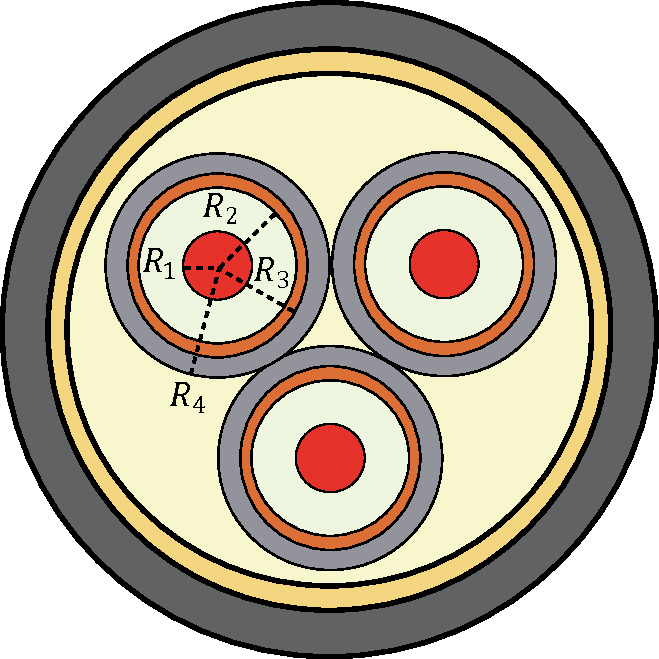
\includegraphics[width = 0.7\columnwidth]{cabo_v4.pdf}
    \caption{Detailed Cross-Sectional View of the Simulated Pipe-Type (PT) Cable. Adapted from \cite{LI2022377}.}
    \label{fig:cable}
\end{figure}

\section{Frequency-Domain propagation for the MTL}
\subsection{Decoupling the MTL Equations by Similarity Transformations}



%%%%%%%%%

In the context of wave equation solutions, the series impedance is defined as $\hat{\mathbf{Z}}=\mathbf{R}+j \omega \mathbf{L}$, and the shunt admittance as $\hat{\mathbf{Y}}=\mathbf{G}+j \omega \mathbf{C}$. Solving this involves addressing a second-order system of coupled differential equations, represented as:
\begin{equation}
\frac{d^2}{d z^2} \hat{\mathbf{V}}(z) =\hat{\mathbf{Z}} \hat{\mathbf{Y}} \hat{\mathbf{V}}(z) \qquad 
\frac{d^2}{d z^2} \hat{\mathbf{I}}(z) =\hat{\mathbf{Y}} \mathbf{Z} \mathbf{\mathbf { I }}(z)
\end{equation}

This system is reformulated into $n$ distinct equations that describe $n$ isolated two-conductor lines, as per \cite{Paul2007}. The conversion between phase and modal quantities is expressed through $\hat{\mathbf{V}}(z) =\hat{\mathbf{T}}_V \hat{\mathbf{V}}_{\mathrm{m}}(z)$ and $\hat{\mathbf{I}}(z) =\hat{\mathbf{T}}_I \hat{\mathbf{I}}_{\mathrm{m}}(z)$. The $n \times n$ complex matrices $\hat{\mathbf{T}}_V$ and $\hat{\mathbf{T}}_I$ facilitate a variable transformation between the actual phasor line voltages and currents, $\hat{\mathbf{V}}$ and $\hat{\mathbf{I}}$, and the modal voltages and currents, $\hat{\mathbf{V}}_{\mathrm{m}}$ and $\hat{\mathbf{I}}_{\mathrm{m}}$:
\begin{equation}
\begin{gathered}
\frac{d^2}{d z^2} \hat{\mathbf{V}}_{\mathrm{m}}(z)  =\hat{\mathbf{T}}_V^{-1} \hat{\mathbf{Z}} \hat{\mathbf{Y}} \hat{\mathbf{T}}_V \hat{\mathbf{V}}_{\mathrm{m}}(z) =\hat{\gamma}^2 \hat{\mathbf{V}}_{\mathrm{m}}(z) \\  
\frac{d^2}{d z^2} \hat{\mathbf{I}}_{\mathrm{m}}(z)  =\hat{\mathbf{T}}_I^{-1} \hat{\mathbf{Y}} \hat{\mathbf{Z}} \hat{\mathbf{T}}_I \hat{\mathbf{I}}_{\mathrm{m}}(z) =\hat{\gamma}^2 \hat{\mathbf{I}}_{\mathrm{m}}(z)
\end{gathered}   
\end{equation}

%%%%%%%%%


The mode equations will therefore be decoupled. This will yield the $n$ propagation constants $\hat{\gamma}_i$ of the $n$ modes. Thus, the equations governing the mode voltages and currents have the simple solution:
\begin{equation}
\begin{gathered}
\hat{\mathbf{V}}_{\mathrm{m}}(z)=\mathbf{e}^{-\hat{\gamma} z} \hat{\mathbf{V}}_{\mathrm{m}}^{+}+\mathbf{e}^{\hat{\gamma} z} \hat{\mathbf{V}}_{\mathrm{m}}^{-}  \\ \hat{\mathbf{I}}_{\mathrm{m}}(z)=\mathbf{e}^{-\hat{\gamma} z} \hat{\mathbf{I}}_{\mathrm{m}}^{+}-\mathbf{e}^{\hat{\gamma} z} \hat{\mathbf{I}}_{\mathrm{m}}^{-}    
\end{gathered}
\end{equation}

\begin{figure*}[t!]
\centering
\includegraphics[width=\textwidth]{PSCAD.png}
\caption{The PSCAD model used in case studies includes phasor measurement units for voltage and current in both terminals. These measurements cover not only the phases but also the shields and pipes.}
\label{PSCAD}
\end{figure*}


\subsection{Characterizing the Line as a 2n-Port with the Chain-Parameter Matrix}

Since we are focused on the terminal voltages and currents, employing a Chain-Matrix that relates the voltages and currents at the input and output of the cable is advantageous \cite{Paul2007}. To construct such a matrix, we first define the characteristic impedance and admittance of the Multiconductor Transmission Line (MTL) as follows:
\begin{equation}
\hat{\mathbf{Z}}_{\mathrm{C}}=\hat{\mathbf{Y}}^{-1} \hat{\mathbf{T}}_I \hat{\gamma} \hat{\mathbf{T}}_I^{-1} \qquad \hat{\mathbf{Y}}_C = \hat{\mathbf{T}}_I \hat{\gamma}^{-1} \hat{\mathbf{T}}_I^{-1} \hat{\mathbf{Y}}
\end{equation}
The Equation \ref{matriz_PHI} represents the chain matrix,
\begin{equation}
\begin{aligned}
{\left[\begin{array}{l}
\hat{\mathbf{V}}(\mathscr{L}) \\
\hat{\mathbf{I}}(\mathscr{L})
\end{array}\right] } & =\left[\begin{array}{ll}
\hat{\Phi}_{11}(\mathscr{L}) & \hat{\Phi}_{12}(\mathscr{L}) \\
\hat{\Phi}_{21}(\mathscr{L}) & \hat{\Phi}_{22}(\mathscr{L})
\end{array}\right]\left[\begin{array}{l}
\hat{\mathbf{V}}(0) \\
\hat{\mathbf{I}}(0)
\end{array}\right]
\end{aligned}
\label{matriz_PHI}
\end{equation}
where each block of the Chain-Matrix is defined as follows, termed  $\hat{\mathbf{M}} = \sqrt{\hat{\mathbf{Z}} \hat{\mathbf{Y}}} \mathscr{L}$.
\begin{equation*}
\hat{\Phi}_{11}(\mathscr{L})  =\cosh \left( \hat{\mathbf{M}} \right) \qquad \hat{\Phi}_{12}(\mathscr{L}) =-\sinh \left( \hat{\mathbf{M}} \right) \hat{\mathbf{Z}}_{\mathrm{C}}
\end{equation*}
\begin{equation*}
\hat{\Phi}_{21}(\mathscr{L}) =-\hat{\mathbf{Y}}_{\mathrm{C}} \sinh \left( \hat{\mathbf{M}} \right)  ~ \hat{\Phi}_{22}(\mathscr{L}) = \hat{\mathbf{Y}}_{\mathrm{C}} \cosh \left( \hat{\mathbf{M}} \right) \hat{\mathbf{Z}}_{\mathrm{C}}
\end{equation*}

If the line is heterogeneous, the Chain-Matrix can be obtained by the product of each segment with distinct properties, taking care to maintain the correct order in the matrix multiplication.
\begin{equation*}
\begin{aligned}
\hat{\Phi}(\mathscr{L}) & =\hat{\Phi}_N\left(\Delta z_N\right) \times \cdots \times \hat{\Phi}_i\left(\Delta z_i\right) \times \cdots \times \hat{\Phi}_1\left(\Delta z_1\right) \\
& =\prod_{k=1}^N \hat{\Phi}_{N-k+1}\left(\Delta z_{N-k+1}\right)
\end{aligned}
\end{equation*}

It should be noted that this approach allows for the consideration of cable twisting, as well as phase transposition and the cross-bonding of shields. 

\subsection{Incorporating the Terminal Conditions}

To determine the terminal voltages, it's necessary to consider the terminal conditions, which are the generalized Thévenin equivalents at the input and output of the 2n-port circuit. Here, $\hat{\mathbf{V}}_{\mathrm{S}}$ and $\hat{\mathbf{Z}}_{\mathrm{S}}$ pertain to the generator side, and $\hat{\mathbf{V}}_{\mathrm{L}}$ and $\hat{\mathbf{Z}}_{\mathrm{L}}$ to the load side. For the same Chain Matrix $\hat{\Phi}$, we incorporate these terminal conditions when solving a linear system of the type $\mathbf{A} = \mathbf{x} \mathbf{b}$, where
\begin{equation}
\mathbf{A} = \left[\hat{\Phi}_{12}-\hat{\Phi}_{11} \hat{\mathbf{Z}}_{\mathrm{S}}-\hat{\mathbf{Z}}_{\mathrm{L}} \hat{\Phi}_{22}+\hat{\mathbf{Z}}_{\mathrm{L}} \hat{\Phi}_{21} \hat{\mathbf{Z}}_{\mathrm{S}}\right]   
\end{equation}
and
\begin{equation}
\mathbf{x} = \hat{\mathbf{I}}(0) \qquad \mathbf{b} = \hat{\mathbf{V}}_{\mathrm{L}}-\left[\hat{\Phi}_{11}-\hat{\mathbf{Z}}_{\mathrm{L}} \hat{\Phi}_{21}\right] \hat{\mathbf{V}}_{\mathrm{S}}
\end{equation}

%%%%
This allows for the calculation of $\hat{\mathbf{I}}(0)$ and subsequently the current at the cable end:

\begin{equation}
\mathbf{I}(\mathscr{L})=\hat{\Phi}_{21} \hat{\mathbf{V}}_{\mathrm{S}}+\left[\hat{\Phi}_{22}-\hat{\Phi}_{21} \hat{\mathbf{Z}}_{\mathrm{S}}\right] \hat{\mathbf{I}}(0)
\end{equation}

We can then determine other essential quantities for analysis, such as the voltage at the cable ends.

\begin{equation}
\begin{aligned}
&\hat{\mathbf{V}}(0)=\hat{\mathbf{V}}_{\mathrm{S}}-\hat{\mathbf{Z}}_{\mathrm{S}} \hat{\mathbf{I}}(0),\\
&\hat{\mathbf{V}}(\mathscr{L})=\hat{\mathbf{V}}_{\mathrm{L}}+\hat{\mathbf{Z}}_{\mathrm{L}} \hat{\mathbf{I}}(\mathscr{L})
\end{aligned}
\end{equation}

With this approach, all terminal voltages and currents are calculated simultaneously. If the cable exhibits parameter variations along its length, the matrix $\hat{\Phi}$ can be modified by the product of the segments, and then the terminal conditions can be applied as done for a simple homogeneous section.
%%%%

\begin{table*}[t!]
\tiny % Reduce the font size
\centering
\caption{Series impedance matrix (Z) in $\Omega/m$}
\label{tab:Z}
\begin{tabular}{crrrrrrr}
\toprule
 & Phase 1 & Shield 1 & Phase 2 & Shield 2 & Phase 3 & Shield 3 & Pipe \\
\midrule
Phase 1 & 1.0449e-04 + 8.4750e-04j & 6.2277e-05 + 7.2861e-04j & 5.7775e-05 + 6.8597e-04j & 5.7775e-05 + 6.8597e-04j & 5.7775e-05 + 6.8597e-04j & 5.7775e-05 + 6.8597e-04j & 5.9612e-05 + 6.7291e-04j \\
Shield 1 & 6.2277e-05 + 7.2861e-04j & 9.0938e-05 + 7.2763e-04j & 5.7775e-05 + 6.8597e-04j & 5.7775e-05 + 6.8597e-04j & 5.7775e-05 + 6.8597e-04j & 5.7775e-05 + 6.8597e-04j & 5.9612e-05 + 6.7291e-04j \\
Phase 2 & 5.7775e-05 + 6.8597e-04j & 5.7775e-05 + 6.8597e-04j & 1.1290e-04 + 8.3071e-04j & 6.7500e-05 + 7.0665e-04j & 5.6807e-05 + 6.7820e-04j & 5.6807e-05 + 6.7820e-04j & 5.9612e-05 + 6.7291e-04j \\
Shield 2 & 5.7775e-05 + 6.8597e-04j & 5.7775e-05 + 6.8597e-04j & 6.7500e-05 + 7.0665e-04j & 9.6161e-05 + 7.0567e-04j & 5.6807e-05 + 6.7820e-04j & 5.6807e-05 + 6.7820e-04j & 5.9612e-05 + 6.7291e-04j \\
Phase 3 & 5.7775e-05 + 6.8597e-04j & 5.7775e-05 + 6.8597e-04j & 5.6807e-05 + 6.7820e-04j & 5.6807e-05 + 6.7820e-04j & 1.1290e-04 + 8.3071e-04j & 6.7500e-05 + 7.0665e-04j & 5.9612e-05 + 6.7291e-04j \\
Shield 3 & 5.7775e-05 + 6.8597e-04j & 5.7775e-05 + 6.8597e-04j & 5.6807e-05 + 6.7820e-04j & 5.6807e-05 + 6.7820e-04j & 6.7500e-05 + 7.0665e-04j & 9.6161e-05 + 7.0567e-04j & 5.9612e-05 + 6.7291e-04j \\
Pipe & 5.9612e-05 + 6.7291e-04j & 5.9612e-05 + 6.7291e-04j & 5.9612e-05 + 6.7291e-04j & 5.9612e-05 + 6.7291e-04j & 5.9612e-05 + 6.7291e-04j & 5.9612e-05 + 6.7291e-04j & 8.4253e-05 + 6.7228e-04j \\
\bottomrule
\end{tabular}
\end{table*}

\begin{table*}[t!]
\tiny % Reduce the font size
\centering
\caption{Shunt admittance matrix (Y) in $\mho/m$}
\label{tab:Y}
\begin{tabular}{crrrrrrr}
\toprule
 & Phase 1 & Shield 1 & Phase 2 & Shield 2 & Phase 3 & Shield 3 & Pipe \\
\midrule
Phase 1 & 0.0000e+00 + 4.8455e-08j & 0.0000e+00 + -4.8455e-08j & 0.0000e+00 + 0.0000e+00j & 0.0000e+00 + 0.0000e+00j & 0.0000e+00 + 0.0000e+00j & 0.0000e+00 + 0.0000e+00j & 0.0000e+00 + 0.0000e+00j \\
Shield 1 & 0.0000e+00 + -4.8455e-08j & 0.0000e+00 + 1.4170e-07j & 0.0000e+00 + 0.0000e+00j & 0.0000e+00 + -4.5602e-08j & 0.0000e+00 + 0.0000e+00j & 0.0000e+00 + -4.5602e-08j & 0.0000e+00 + -2.0445e-09j \\
Phase 2 & 0.0000e+00 + 0.0000e+00j & 0.0000e+00 + 0.0000e+00j & 0.0000e+00 + 4.8455e-08j & 0.0000e+00 + -4.8455e-08j & 0.0000e+00 + 0.0000e+00j & 0.0000e+00 + 0.0000e+00j & 0.0000e+00 + 0.0000e+00j \\
Shield 2 & 0.0000e+00 + 0.0000e+00j & 0.0000e+00 + -4.5602e-08j & 0.0000e+00 + -4.8455e-08j & 0.0000e+00 + 2.6033e-07j & 0.0000e+00 + 0.0000e+00j & 0.0000e+00 + -4.1933e-08j & 0.0000e+00 + -1.2434e-07j \\
Phase 3 & 0.0000e+00 + 0.0000e+00j & 0.0000e+00 + 0.0000e+00j & 0.0000e+00 + 0.0000e+00j & 0.0000e+00 + 0.0000e+00j & 0.0000e+00 + 4.8455e-08j & 0.0000e+00 + -4.8455e-08j & 0.0000e+00 + 0.0000e+00j \\
Shield 3 & 0.0000e+00 + 0.0000e+00j & 0.0000e+00 + -4.5602e-08j & 0.0000e+00 + 0.0000e+00j & 0.0000e+00 + -4.1933e-08j & 0.0000e+00 + -4.8455e-08j & 0.0000e+00 + 2.6033e-07j & 0.0000e+00 + -1.2434e-07j \\
Pipe & 0.0000e+00 + 0.0000e+00j & 0.0000e+00 + -2.0445e-09j & 0.0000e+00 + 0.0000e+00j & 0.0000e+00 + -1.2434e-07j & 0.0000e+00 + 0.0000e+00j & 0.0000e+00 + -1.2434e-07j & 0.0000e+00 + 1.6065e-06j \\
\bottomrule
\end{tabular}
\end{table*}


\section{Case Studies}

In this section, we will perform a comparative analysis between the results obtained from steady-state PSCAD simulations and those derived from the methodology detailed in this paper. We will explore four distinct scenarios: simulating the cable with both shields and pipes grounded at both ends, simulating with only the emitter side grounded while leaving the load side open, investigating voltage drop in a cable with the same cross-section but varying lengths, and analyzing the voltages along the cable length. The cable parameters were determined using PSCAD, and the series impedance and shunt admittance matrices are presented in Tables \ref{tab:Z} and \ref{tab:Y}. These same values were incorporated into the proposed software.

The PSCAD model, illustrated in Figure \ref{PSCAD}, utilizes Phasor Measurement Units (PMUs) to evaluate voltage and current at both terminals of the cable. Notably, the analysis expands beyond phase assessment to include a comprehensive examination of shields and pipes, establishing a robust analytical framework.

For accurate comparisons, we derived cable parameters from PSCAD simulations, while Pipe-Type cable parameters were obtained using analytical formulas as outlined in \cite{Ametani2015}. The series impedance and shunt admittance were exported as matrices, and we employed the multi-conductor transmission line software developed by the authors to conduct the analysis.

For the case studies, the cable operates within an ideal unitary three-phase system and is submerged in a marine environment with a seabed resistivity of \(\rho_{\text{seabed}} = 100 \, \Omega \cdot m\) at a depth of 1 m. The system includes a load of 1$\Omega$ per phase and a resistance of 1 m$\Omega$ at the shields when grounded, and 1k$\Omega$ when the terminal is not grounded. The first two case studies use a length of 1 km and the third cases study varies the cable length.

The cable, as illustrated in Figure \ref{fig:cable}, comprises several coaxial layers with radii \(R_1 = 11.75 \, \text{mm}\), \(R_2 = 43.05 \, \text{mm}\), \(R_3 = 46.55 \, \text{mm}\), and \(R_4 = 49.85 \, \text{mm}\). Its design incorporates a copper conductor and XLPE insulation (\(\varepsilon_r = 2.2\)). Additionally, the cable features a 6 mm non-magnetic pipe (\(\rho_s = 9.78 \times 10^{-8} \, \Omega \cdot m\)), along with internal and external dielectric layers having radii of 10.955 cm and 11.955 cm, respectively, employing an insulator with the same permittivity as the coaxial layers.

\subsection{Grounded shields at both terminals}

This case study concentrates on terminal voltages and currents. In this scenario, we ground every shield at both ends, a condition also applied to the pipe conductor. This setup serves as the basis for the last two case studies in this section: one involving varying cable lengths, and the other calculating voltages and currents along the conductor. In this configuration, significant currents flow through the shield conductors, resulting in considerable resistive losses that affect the cable's ampacity.

The analysis aims to comprehend the impact of these conditions on the submarine cable system's performance and efficiency. We utilized the PSCAD software to analyze steady-state voltage and current characteristics, comparing them with our method. The summarized findings from both analyses are shown in Table \ref{tab:results}. The PSCAD setup is according to Fig. \ref{PSCAD}.
In this case study, we observe a perfect match between the two approaches, indicating the validity of our method.

\begin{table}[h]
    \centering
    \caption{Comparative Analysis of Selected Voltages and Currents}
    \begin{tabular}{@{}ccc@{}}
    \toprule
    & \textbf{PSCAD} & \textbf{Proposed} \\
    \midrule
    \(I_{\text{pipe}} (z=0)\) & \(0.1365 \angle -157.20^\circ\) & \(0.1364 \angle -157.20^\circ\) \\
    \(I_{\text{sheat}1} (z=0)\) & \(0.6746 \angle 29.85^\circ\) & \(0.6744 \angle 29.87^\circ\) \\
    \(I_{\text{sheat}2} (z=0)\) & \(0.5805 \angle -89.03^\circ\) & \(0.5804 \angle -89.03^\circ\) \\
    \(I_{\text{sheat}3} (z=0)\) & \(0.5532 \angle 148.20^\circ\) & \(0.5531 \angle 148.21^\circ\) \\
    \(V_1 (z=\mathscr{L})\) & \(0.9359 \angle -7.08^\circ\) & \(0.9360 \angle -7.08^\circ\) \\
    \(V_2 (z=\mathscr{L})\) & \(0.9385 \angle -127.00^\circ\) & \(0.9385 \angle -127.01^\circ\) \\
    \(V_3 (z=\mathscr{L})\) & \(0.9388 \angle 113.10^\circ\) & \(0.9389 \angle 113.05^\circ\) \\
    \bottomrule
    \end{tabular}
    \label{tab:results}
\end{table}

\subsection{Shields grounded at the source end and left open at the load end}

In this scenario, the cable shields are grounded at the source end but left open at the load end, while the armor is grounded at both ends.

Table \ref{tab:results_case2} presents the results for armor and sheath currents, as well as the terminal phase voltages obtained from our proposed method, compared with those from PSCAD. In the results of our proposed method, there is a slight imbalance in voltages, likely because our model does not consider phase transposition.

\begin{table}[h]
    \centering
    \caption{Comparative Analysis of Selected Voltages and Currents}
    \begin{tabular}{@{}ccc@{}}
    \toprule
    & \textbf{PSCAD} & \textbf{Proposed} \\
    \midrule
    \(I_{\text{pipe}} (z=0)\) & \(0.0248605 \angle -96.89^\circ\) & \(0.0211559 \angle 91.43^\circ\) \\
    \(I_{\text{sheat}1} (z=0)\) & \( \text{8.70408E-5} \angle 29.85^\circ\) & \( \text{8.71051E-5} \angle -97.30^\circ\) \\
    \(I_{\text{sheat}2} (z=0)\) & \( \text{7.27377E-5} \angle -89.03^\circ\) & \( \text{7.24579E-5} \angle 144.94^\circ\) \\
    \(I_{\text{sheat}3} (z=0)\) & \( \text{7.12441E-5} \angle -164.4^\circ\) & \( \text{7.09180E-5} \angle 15.33^\circ\) \\
    \(V_1 (z=\mathscr{L})\) & \(0.95032 \angle -9.251^\circ\) & \(0.94393 \angle -8.742^\circ\) \\
    \(V_2 (z=\mathscr{L})\) & \(0.95032 \angle -129.3^\circ\) & \(0.94353 \angle -128.1^\circ\) \\
    \(V_3 (z=\mathscr{L})\) & \(0.95032 \angle 110.7^\circ\) & \(0.93282 \angle 112.1^\circ\) \\
    \bottomrule
    \end{tabular}
    \label{tab:results_case2}
\end{table}

\subsection{Cable voltage drop simulation}

The proposed methodology facilitates the analysis of voltage drop across phase conductors relative to cable length. Figure \ref{fig:dropV} illustrates the voltage magnitude for the three power conductors within the cable. In this scenario, where all shields are grounded at both ends. There are three curves to illustrate the voltage magnitudes. These curves are superimposed because the voltages are perfectly balanced in this case.

Such an investigation is crucial for understanding the interplay between cable parameters, shield grounding, and load impact on voltage drop. As depicted in the figure, certain cable lengths are impractical under these constructional conditions.
\begin{figure}[h!]    
    \centering
    %\includegraphics[width = 0.75\columnwidth]{cabo_artigo.pdf}
    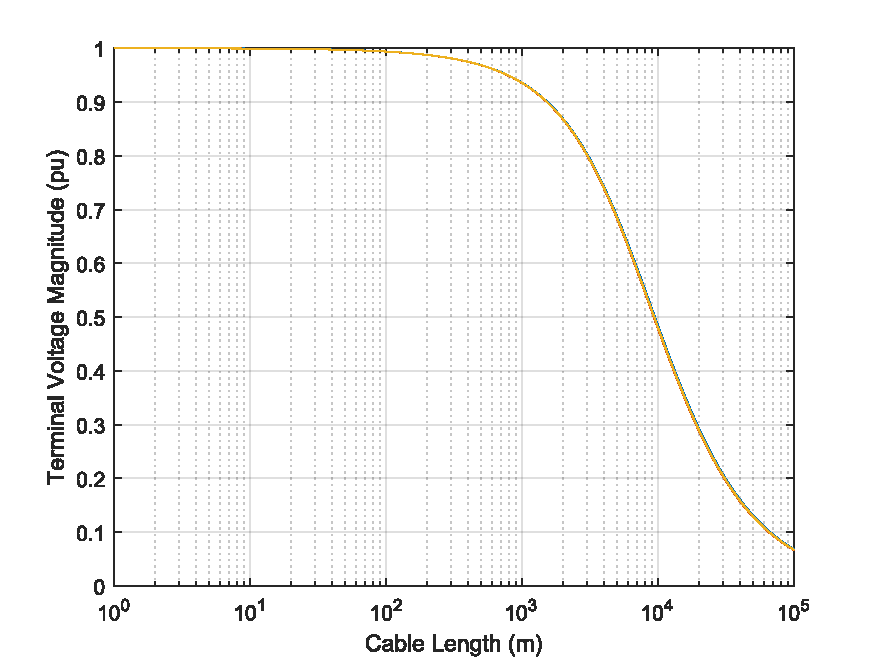
\includegraphics[width = \columnwidth]{drop_voltage.pdf}
    \caption{ Terminal voltage at the load side as a function of the cable lengh.}
    \label{fig:dropV}
\end{figure}

\subsection{Voltages and currents along the cable}

The proposed methodology expands the ability to analyze voltages and currents along the cable's length, moving beyond the conventional focus solely on terminals. Figure \ref{fig:shields} demonstrates the voltage magnitude and amplitude of the shield conductors and the pipe. In the configuration under examination, each terminal is grounded, enabling the identification of a point of zero voltage on the shield and armor conductor. This zero voltage point is often chosen for cable splices due to its unique characteristic. Through simulation using the proposed solution, such a point can be accurately determined.

\begin{figure}[h!]    
    \centering
    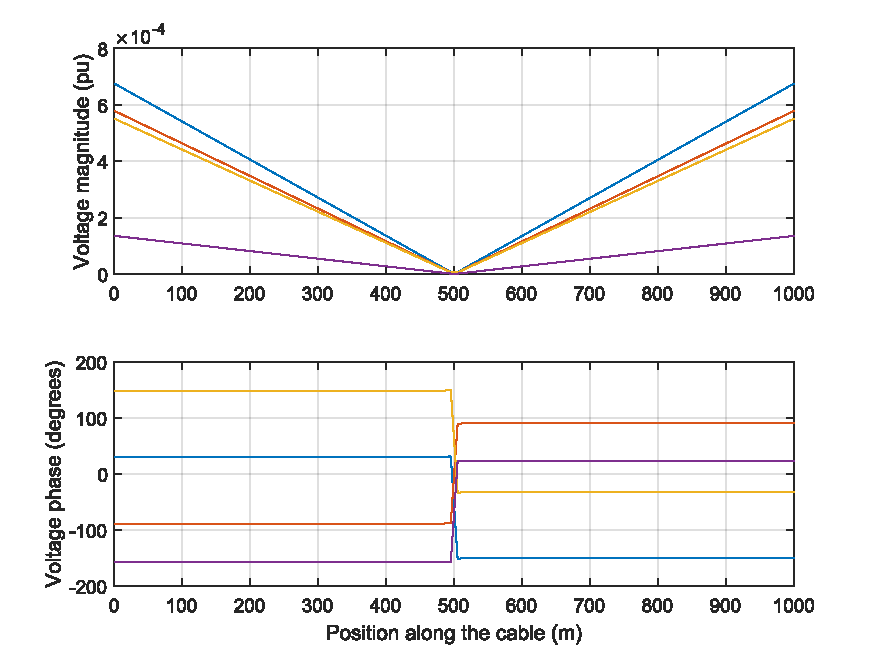
\includegraphics[width = \columnwidth]{shields.pdf}
    \caption{ Voltage magnitude and phase of shield conductors and the pipe.}
    \label{fig:shields}
\end{figure}



\subsection{Conclusion}

The PT Cable simulation, based on parameters obtained with PSCAD, was validated by comparing it with the same software's results. This method efficiently captures steady-state conditions, avoiding the intensive computations of traditional time-domain solutions. It's particularly effective for analyzing voltage drops and sheath currents in the cable, providing precise results with reduced computational effort, thus making the analysis process more efficient.



\vfill


% use section* for acknowledgement
\section*{Acknowledgement}

We gratefully acknowledge the support of the RCGI – Research Centre for Greenhouse Gas Innovation (23.1.8493.1.9), hosted by the University of São Paulo (USP), sponsored by FAPESP – São Paulo Research Foundation (2020/15230-5), and sponsored by TotalEnergies, and the strategic importance of the support given by ANP (Brazil’s National Oil, Natural Gas and Biofuels Agency) through the R\&DI levy regulation.

\bibliographystyle{IEEEtran}
\bibliography{IEEEabrv,refs}







\end{document}

